\documentclass[a4j,10pt]{jsarticle}
\usepackage{layout,url,resume}
\usepackage[dvipdfmx]{graphicx}
\usepackage[dvipdfmx]{hyperref}
\pagestyle{empty}

\begin{document}
%\layout

\title{小型ハイブリッドロケット向けフライトシミュレータの開発}

% 和文著者名
\author{
	Arch B1 坂本優太(sksat)
}

% 和文概要
\begin{abstract}
小型ハイブリッドロケットを対象としたフライトシミュレータを新規に開発した.
\end{abstract}

\maketitle
\thispagestyle{empty}

\section{開発の経緯}
% COREとかいうのに入ってる
% ハイブリッドロケット is 何
% 安全審査 is 何

筆者は"CORE"\footnote{"Challengers Of Rocket Engineering"の頭文字をとったもの.}
という学生ロケット
\footnote{「学生ロケット」という言葉には明確な定義は無いが,ここでは学生を主体とした小型のロケットの開発・打ち上げ活動とする.}
サークルに所属している.
COREでは主に小型ハイブリッドロケットの開発・打ち上げ実験を行っている.

これらのロケットを設計する際,
ロケットがどのように・どの程度飛翔すかといった検討を行う.
ロケットの飛翔を解析的に解くのは難しい
\footnote{ロケットはその性質上,質量・推力を刻一刻と変化させながら飛翔する上に,
空力による影響が大きい.解析的に解くのはとても大雑把な検討をする際のみであろう.}
ため,コンピュータを使って数値計算(以後シミュレーションと呼称)を行う必要がある.
また,このシミュレーションはロケットを打ち上げるにあたって事前・直前に実施される安全審査においても要求されるものとなっており,
打上における安全確保の観点からも重要なものである.

このシミュレーションを行うために,
COREでは過去にOBが開発したシミュレータ"FROGS"
\footnote{Flight Of ROcket and Ground-hit-points Simulator.}
を使用してきた.
しかし,筆者がシミュレーション担当となり,
8,11月の打上実験においてFROGSを使用したところ,様々な問題点があることが分かった.
これらの問題点を解消するため,今回新たなフライトシミュレータを開発するに至った.

% ハイブリッドロケットは液体燃料ロケット・固体燃料ロケットと並ぶ化学反応を利用した種類のロケット推進システムの1つである.
% ハイブリッドロケットが「ハイブリッド」と呼ばれる所以は,
% 相の異なる2種類の推進剤を用いるという特徴にある.
% 最も多いのは液体の酸化剤と固体の燃料を用いる方式であり,
% これはいわば液体燃料ロケットと固体燃料ロケットを足して2で割ったようなものだ.
% 実際に,ハイブリッドロケットは双方のロケットシステムの利点を兼ね備えている.
% 
% ハイブリッドロケットは本質的に爆発しないと言われており,
% その他のロケットに比べ安全性が高い.
% そのため,大学生でも扱うことができるよん.

\section{既存のシミュレータの問題点}

% FROGSが如何にカスか
% matlabだとインカレで困る
% コードがカス: 関数なにそれおいしいの
% パラメータ入力がカス
% 可視化もカス

まず重要なこととして,FROGSがMATLAB向けに書かれたプログラムだということが挙げられる.
COREはインターカレッジ・サークルであり,首都大学東京
\footnote{2020年4月以降"東京都立大学"に改称予定.}
を中心とした様々な大学の学生が集まった団体となっている.
なので,中にはMATLABのライセンスを学生に配布していない大学の学生もいる.
MATLABのライセンスは一介の大学生に購入できるものではないため,
必然的にCORE内でFROGSを使うことができる人間は限られてしまう.

また,FROGSはあまりソフトウェア開発の経験が無い人によって開発・保守されてきた.
このため,パラメータの入力が配列への直接代入であるなど,
コードの再利用性が著しく低い上,
Google Drive上でフォルダ名によってバージョン管理がなされている,
といった運用状況があった.

これは個人的に許容できるものではなかったため,
文字コードの変更やインデントの修正を行ったものをGitに取り込み,
https://github.com/core-rocket/FROGS
\footnote{そもそも,https://github.com/core-rocket というorganizationも筆者が作成・整備したものだ.}
にて公開した.
2019年11月の伊豆大島共同打上実験と,
現在プロジェクトが進行中の2020年3月の伊豆大島共同打上実験において
筆者が担当するシミュレーションはこのリポジトリで行っている.

さらに,計算結果の可視化に関しても,FROGSには問題があった.
まず,計算結果のファイル保存を行わないため,
可視化を行うためには毎回計算を実行しなければならなかった.
1ケースのみの可視化をしたい場合であれば,
計算時間も短いのでこれは大した問題にはならない.
だが,次に述べる落下分散図の作成時や,再計算を要求された時など,
複数のケースを検討する必要がある場合,
FROGSではこれは根気の要る作業となる.

落下分散図は,小型ハイブリッドロケットでは(特に安全審査において)最も重要な可視化である.
これは,ある条件
\footnote{ランチャの仰角が何度か,パラシュートが正常に開いた場合や開かずロケットが弾道してしまった場合,といったものが実際に検討する条件となる.}
でロケットを発射した際に,
ロケットが落下する地点の座標を複数の風向・風速毎に,
図\ref{ghp-example}のようにプロットしたものだ.

\begin{figure}[htbp]
	\begin{center}
		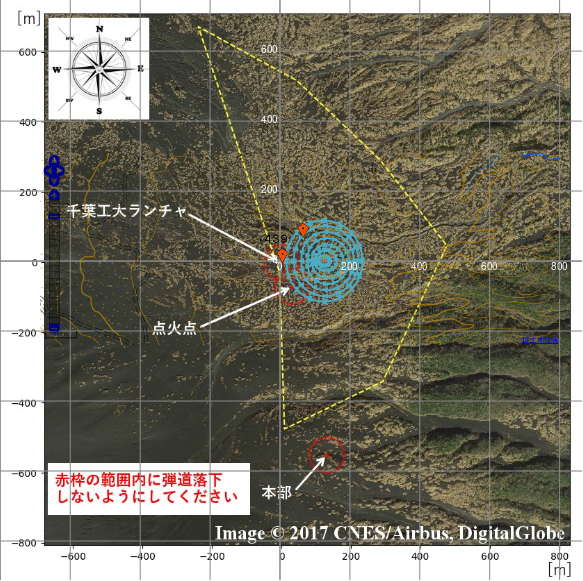
\includegraphics[width=7cm]{./ghp-example.png}
		\caption{落下分散図の例}
		\label{ghp-example}
	\end{center}
\end{figure}

どのようなロケットにおいても,
それが上空から落下してくる可能性がある以上,
「ここに落としてはいけない」という落下禁止区域が存在する.
落下禁止区域は土地の所有者や漁協との兼ね合いに加え,
打上関係者を含む全ての人間の安全のために設定される.

FROGSでは,この落下分散図を作るために,いわゆる「神Excel」のようなものを用いていた.
図\ref{ghp-example}を良く見ると,地図の画像の上に罫線があるのが分かるが,
これはExcelのセルなのである.
このExcelファイルは特定のセルに落下地点の座標群(以後GHP: Ground-Hit-Point)を入れると,
地図の画像が貼り付けられている部分のセル上に点をプロットするように作られている.
そして,実際の可視化の際はFROGSで落下分散を計算した後,
MATLABの変数のタブからGHPの行列を選択し,値を全てコピー,
ExcelファイルのGHPのセルにペースト,という手順を踏まねばならない.

そして,もちろんこのExcelファイルは実験の度に落下禁止区域の画像を元にして作り直さねばならない.
このような可視化は非常に面倒である上に,
正確性を欠くため,改善する必要性があった.

\section{先行事例}
% FROGS, ForRocket, OpenTsiolokvsky
% OpenRocketは先行事例 && 先行研究みがある
% OpenRocketはプロトタイプには良いが

COREのFROGS以外にも,多くの学生ロケット団体が独自にシミュレータを開発している.
しかし,学生ロケットの分野においてはまだオープンソースの文化が浸透していない.
そのため,挙げられる先行事例は多くない.

ForRocketは他団体のOBが開発しているもので,
Pythonで書かれている.
今回シミュレータをフルスクラッチするにあたって大いに参考になった技術同人誌
\ref{hybrid-rocket-know-how}のうち,シミュレーションに関する記述はForRocketの開発者によるものだ.

OpenTsiolokvskyはサウンディングロケット"MOMO"の開発・打上を行っている
インターステラテクノロジズ社のシミュレータで,実際にMOMOの開発時に使われているらしい.
MOMOはハイブリッドロケットではなく液体燃料ロケットだが,参考にできる部分は大きいだろう.
シミュレータ本体はC++,可視化部分などはPythonで書かれている.

また,小型ハイブリッドロケットや液体燃料ロケットではなく,
モデルロケットという小型の固体燃料ロケットを対象にしたシミュレータも存在する.
このようなシミュレータのうち,オープンソースで代表的なものはOpenRocketである.
\footnote{シミュレータというよりは設計とシミュレーションを行うための統合環境なのだが,
シミュレータ部分で行っていることはハイブリッドロケットのシミュレーションと似たようなものであるため,先行事例とした.}
小さなモデルロケットの設計・シミュレーションには申し分ないソフトウェアとなっており,
小型ハイブリッドロケットの設計・シミュレーションも可能ではあるため,
小型ハイブリッドロケット開発ではプロトタイプの検討に使われることが多い.
だが,圧力中心の計算がポテンシャル流れを仮定したものである他,
フィンに台形以外の形状を使用した際に著しく正確性を欠くなどの問題点があり,
伊豆大島共同打ち上げ実験・能代宇宙イベントでは推奨されていない.
元はヘルシンキ大学の修士論文
\footnote{Development of an Open Source model rocket simulation
software}
のためのプロジェクトであり,先行研究とも言える.


\section{実装}

\subsection{シミュレータ本体}

実装にはC++17を使用した.
\footnote{今後C++20に移行する可能性がある.}

マルチプラットフォームでの動作を目的の1つとしていたため,
使用するライブラリはできるだけ少なくなるようにした.
C++標準のSTL以外で使用したのはEigenとtoml11というライブラリのみである.
これらのライブラリはヘッダオンリライブラリであるため,
バイナリ配布時にdllファイルなどを同梱する必要が無い.
Eigenはベクトル,四元数,行列といった数学的概念を扱うために,
toml11はTOMLファイルの読み込みに使用した.

ソースコード及び,各バージョンのビルド済みバイナリはhttps://github.com/sk2sat/trochiaにて公開している.

\subsubsection{TOMLファイルによるパラメータ入力}
FROGSでは,パラメータの入力は全てFROGS内の変数への代入でしかなかった.
入力するパラメータには,
ロケットの機体の諸元の設計値もしくは実測値,
ランチャ仰角や風向・風速といった環境の情報,
搭載するエンジンの推力履歴がある.

まず,機体の諸元については,
FROGSではPMTという配列にひたすら値を代入していく,という方法を取っていた.
この配列に間違いなく諸元を代入するために,
"諸元コピペ用シート"というExcelファイルが作られていたが,
それは対症療法でしかなく,面倒なことに変わりはない.

そのため,trochiaではTOMLファイルによってパラメータの入力を行うことにした.
% 変数名を明確に指定 ミスも無くせる

次に,環境の情報についてなのだが,
ランチャの仰角は人間が設定できるパラメータ,
風向・風速などは刻一刻と変わるパラメータであり,可変である.
そのため,これらのパラメータを少しずつ変化させて色々な条件でシミュレーションを行うことが可能であり,実際それが求められる.
% 風向風速制限の話

エンジンの推力履歴については,以前はこれも配列への直接代入だったようだが,
途中からMATLABのreadmatrix関数を使うことで,ファイル名を指定するだけでよくなったようだ.
だが,推力の補完などを全く考慮していないため,
もし計算の時間刻みを変えようと思った場合は推力履歴のファイルも作り直す必要があった.
そのため,trochiaでは推力の線形補間を行うように実装したことで,
時間刻みを任意に設定することができるようになった.

\subsubsection{数値積分の改良}
% Euler + RK4 -> RK4 or 色々

FROGSでは,数値積分は回転運動と並進運動に分けて行われていた.
回転運動には4次のRunge-Kutta法(以後RK4),並進運動には1次のオイラー法が用いられていた.
また,数値積分の部分の抽象化や関数化も行っていなかったため,
容易に数値積分法を変更することができなかった.
\footnote{そして,時間刻みも変更することができない.}

そのため,trochiaでは数値積分をその他の計算と分け,抽象化することにした.
まず,double型の変数とその導関数,時間刻みを与えると,
メンバ関数step()を実行する毎に1次のオイラー法で数値積分を実行するクラス
を作成した.
次に,このクラスをtemplateを使って四則演算ができる任意の型を扱えるようにした.
そして,このクラスを抽象化したクラスtrochia::solverを作り,
値の更新を行うメンバ関数step()を純粋仮想関数とした.
これにより,オイラー法などの具体的な数値積分手法を,
step()関数を実装するだけで定義することができ,
それを任意の型から使用することができるようになった.

さらに,回転・並進運動する剛体を考え,これを表現するクラスtrochia::Objectを作り,
ロケットのような物体は全てこのObjectを継承するものとした.
trochia::Objectには導関数を表現するstaticメンバ関数dx()があり,
これは仮想関数なので継承先で書き換えることができる.
trochia::Objectにはいくつかの演算が実装してあるため,
これに対してもtrochia::solverを使うことができる.

現状では1次のEuler法,2次・4次のRunge-Kutta法を実装しており,
デフォルトでは4次のRunge-Kutta法を使用して数値積分を実行するようにしている.

だが,継承を用いた実装の仕方が適切だとはあまり思えないため,
本格的にC++20を導入したらconceptを使って大幅な書き換えをする可能性がある.

\subsubsection{GitHub Actionsを使った自動リリース}

C++を使用する以上,プログラムの実行をするためにはビルドする必要がある.
しかし,プログラミングなどについて知識の無い人でも使うことができるようにしたかったため,
ビルド済みバイナリを配布する必要があった.

そして,trochiaの想定ユーザであるCOREのメンバのほとんどはWindowsかMacを使用している.
筆者は通常Linuxしか使用しないため,
それらの他のプラットフォーム向けにいちいちビルド作業を行うことは困難である.

そのため,今回はGitHub Actionsを用いて,このビルド・リリース作業を自動化した.
GitHub ActionsではプラットフォームとしてUbuntu,Windows,Macをサポートしているため,
クロスコンパイルをせずともそれぞれのプラットフォーム向けにビルドを実行することができる.
元々,trochiaのビルドにはCMakeを用いていたため,
どのプラットフォームでもほぼ同じ手順でビルドを行うことができた.

さらに,こうしてビルドしたバイナリに使用ライブラリのライセンス表示などを追加したものをリリース時に自動でGitHub Releaseにアップロードするようにした.
これにより,Linux,Windows,Macどのプラットフォームにおいても,
GitHub Releaseからビルド済みバイナリをダウンロードしてくるだけでtrochiaを実行することができる.
\footnote{trochiaが使用しているライブラリは標準ライブラリとヘッダオンリライブラリのみであるため,特にランタイムのインストールなどもほぼ必要ない.}

また,この一貫としてCIを整備した結果,
MinGWやVisual C++のC++17のサポート状況の違いがあることが分かった.

\subsection{可視化スクリプト}
% GHPは相対座標
% 落下禁止区域は緯度経度
% pymap3d使って座標変換
% 国土地理院のAPI 地理院タイルを使うと地図がいいかんじに出せてべんり
% leafletでもっとべんり
% GHP -> pymap3d -> js
% js吐くのはアホなのでそのうちjsonに?
% なんか弄ってたら風向風速制限表自動生成できたあ
% 座標変換はそのうちtrochia本体で実装するからこのスクリプトは要らない子になる

可視化手順を改善するにあたり,
今回はシミュレータ本体とは分けて可視化のためのスクリプトをPythonを用いて実装した.
このスクリプトでは,シミュレータが出力したENU座標系
\footnote{射点からの相対座標系で,x軸を東(E),y軸を北(N),z軸を上(U)方向にとったもの.}
のGHPをLLH座標系
\footnote{緯度・経度・高度.}
に変換し,可視化のためのJavaScriptファイルを出力するものとなっている.
座標の変換にはpymap3dというライブラリを用いた.

実際の可視化はJavaScriptの地図ライブラリであるLeafletを用いて行う.
Leafletでは国土地理院の地図APIである地理院タイルを使用して地図の表示を行うことができ,
様々な縮尺・種類の地図を用いることができる.
また,緯度・経度を指定して点や線などを描画することができる.
これを用いて,GHPを図\ref{ghp-new}のように正確かつ簡単に可視化することができるようになった.

さらに,FROGSの方にも手を入れ,GHPをファイルに保存するようにしたことで,
このスクリプトをFROGSからも使用することができるようになった.
これにより,FROGSからtrochiaの移行期間中もこのスクリプトを用いて可視化を行うことができる.

\begin{figure}[htbp]
	\begin{center}
		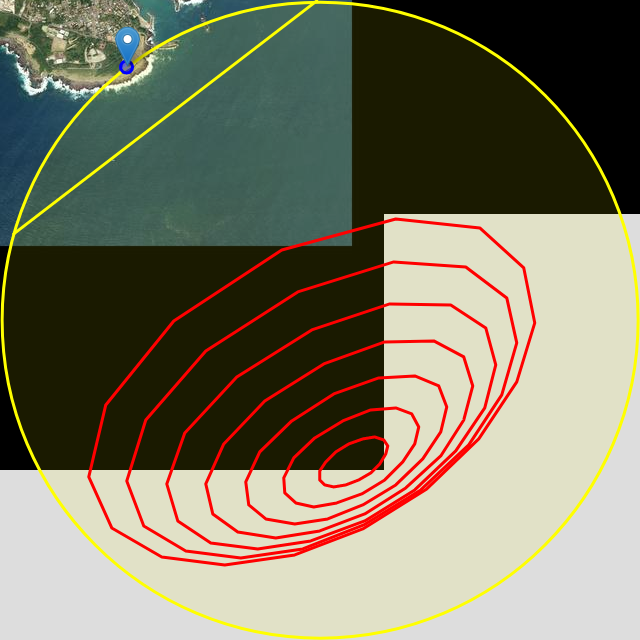
\includegraphics[width=7cm]{./ghp-new.png}
		\caption{今回の実装による落下分散図の例}
		\label{ghp-new}
	\end{center}
\end{figure}

加えて,このスクリプトを拡張することで,
安全審査で求められる図\ref{restrict-table-example}のような風向風速制限表というものをGHPのファイルから自動生成することができるようになった.
風向風速制限表を作るのもこれまでかなりの手間を要していたため,
今回の自動化により,安全審査で提出するシミュレーション計算書の作成が大幅に簡略化された.

\begin{figure}[htbp]
	\begin{center}
		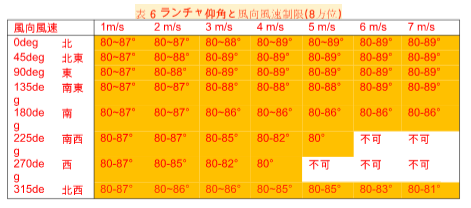
\includegraphics[width=8cm]{./restrict-table-example.png}
		\caption{風向風速制限表の例}
		\label{restrict-table-example}
	\end{center}
\end{figure}

% \subsection{苦労した点}
% MinGWがC++17にちゃんと対応してなくてカス
% Windowsの浮動小数点演算精度が違う
% なんかミスって全部NaN


\section{評価}
\subsection{定性的評価}
% わあい使いやすいね

\begin{table}[htbp]
  \hspace*{-2cm}
  \begin{tabular}{|l|c|c|c|} \hline
         & trochia & FROGS & OpenRocket \\ \hline
	実行に必要なもの & 無し & MATLAB & JRE \\
    コマンドライン実行 & $\bigcirc$ & $\bigtriangleup$ & $\times$ \\
    パラメータ入力 & config.toml & 配列に代入 & GUI \\
	必要な操作数 & $3$ & $2N$ & $\times$ \\
	計算精度 & 標準4次 & 1次+4次 & 4次 \\ \hline
  \end{tabular}
  \caption{定性的評価}
\end{table}

\subsection{定量的評価}
% 高速化
% 近いところに落下分散
% → 頂点到達後しばらくしてから意図しない回転があり,空力まわりにバグ?

今回,定量的に評価を行うことが可能な部分としてシミュレーションの高速化が挙げられる.
この比較はAMD Ryzen 5 3600上のArch Linuxにて行った.
trochiaのビルドにはclang++を用い,最適化オプションにはO2を指定した.
FROGSの実行にはMATLABのR2019bを用いた.

また,計算条件を揃えるため,
入力データには2020年3月の伊豆大島共同打上実験に向けて開発中の機体の諸元と,
同機体に搭載される予定のL型自作エンジン"LIATRIS"の燃焼試験で取得した推力履歴を用いた.

\begin{figure}[htbp]
	\begin{center}
		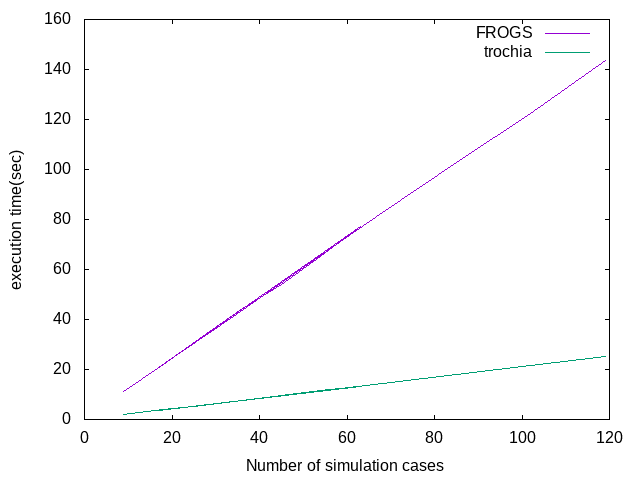
\includegraphics[width=8cm]{./sim-time.png}
		\caption{計算時間の比較}
		\label{sim-time}
	\end{center}
\end{figure}

複数回の計測を行い,図\ref{sim-time}のような結果が得られた.
縦軸が実行にかかった時間,横軸が実行したシミュレーションケースの数となっている.
この結果から,双方のシミュレータによるシミュレーション時間は実行するケースの数にほぼ比例することと,
trochiaのシミュレーションはFROGSと比べ約5.7倍高速だということが分かった.

このような結果が得られた原因としては,
MATLABがインタプリタ型のプログラミング言語であることに加え,
FROGSが無駄なのデータのコピーを多く行っていることが考えられる.

\section{今後}
% バグ修正
% 風向風速制限表の自動生成(できたけど,不十分なのでもうちょいやる)
% FROGS・3月大島データと定量的に比較して妥当性確認
% 燃焼試験データオープンデータ化
% 	既存フォーマットだと不十分,テキストだとサイズがデカい→独自フォーマット考案中
% ペイロード・多段式ロケット実装
% 高度11km以上上空の大気モデル
% マッハ0.8対応
% 精度保証付き数値計算?
% パラメータ最適化

\section{まとめ}

小型ハイブリッドロケットの設計段階及び安全審査において,
筆者の所属する団体"CORE"はFROGSというシミュレータを用いてきたが,
これには様々な問題点があった.
そのため,trochiaという新しいシミュレータの開発を行った.

そして,今回trochiaがそれらの問題点を解消したことと,
trochiaが実際にFROGSよりも優れているということを示した.
今後は,trochiaのシミュレーションの妥当性検証や,
さらなる機能拡張を行っていく予定である.

% \bibliographystyle{junsrt}
% \bibliography{resume}

\begin{thebibliography}{99}
	\bibitem{openrocket-thesis}
		Sampo Niskanen. ; Development of an Open Source model rocket simulation software. (2013-05-20)
	\bibitem{rocket-system}
		田辺英二.ロケットシステム(1999)
	\bibitem{rocket-propulsion-elements}
		George P. Sutton. ; ロケット推進工学.望月晶訳.(1992)
	\bibitem{hybrid-rocket-know-how}
		import Avio.小型ハイブリッドロケットノウハウ vol.1.(2019)
	\bibitem{numerical-calc-common-sense}
		伊里正男,藤野和建.数値計算の常識.(1985)
\end{thebibliography}

\end{document}
% end of file
